\documentclass{beamer}

\title{Decision making using fuzzy soft set inference system}
\author{Saurabh Mathur\\ 
\emph{saurabhmathur96@gmail.com}}

\institute{ SITE, VIT Vellore }
\date{\today}

\usepackage{amsmath}
\usepackage{graphicx}
\begin{document}
  \begin{frame}
    \titlepage
  \end{frame}
  
  
    \begin{frame}
    \tableofcontents
    \end{frame}
    
    
    
  \begin{frame}
  \frametitle{Abstract}
   \begin{LARGE}
    A 5000 feet view
   \end{LARGE}
   \begin{itemize}

   \item Using existing tools in fuzzy set theory to solve problems expressed in terms of soft sets.
   \item  Allowing multiple choices to be made by comparative analysis.
	\item conversion between hybrid fuzzy-soft sets.
   \end{itemize}
  
  \end{frame}
  
  
  \begin{frame}
  \frametitle{Methodology}
    \begin{itemize}
  \item Simulations on Python 2.7 using NumPy.
  \item IPython/Jupyter Notebooks.
  \item Math :)
  \end{itemize}

  \end{frame}
  
  \section{Introduction}
  \frametitle{Introduction}
    \begin{frame}
    \begin{LARGE}
    Dealing with uncertainity
    \end{LARGE}
    \begin{itemize}
        \item theory of probability
    \item interval mathematics
        \item theory of fuzzy sets
    \end{itemize}
    \end{frame}
    
  \begin{frame}
    \frametitle{Soft Sets - Overview}
    \begin{LARGE}
    Soft Sets
    \end{LARGE}
    \begin{itemize}
    	\item Proposed by Molodtsov in 1999 \cite{firstresults}
    	\item A generalization of fuzzy set theory which was given by Zadeh.  
    	\item Aims to solve complicated economic, environmental, and social problems.
    \end{itemize}
  \end{frame}
  
  \begin{frame}
  \frametitle{Soft Sets - Definition}
      \begin{LARGE}
    Definition
    \end{LARGE}
  
    The \emph{soft set} is a parametrized family of subsets of the set $U$. \\
    Every set $F(e)$,
$e \in E$, from this family may be considered as the set of e-elements of the soft set $(F, E)$. \cite{firstresults}
  
  \end{frame}
  
  \begin{frame}
  \frametitle{Soft Sets - Example}
    \begin{LARGE}
    Example
    \end{LARGE}
    
  A soft set $(F, E)$ describes the attractiveness of the houses. \\
$U$ - set of houses under consideration.\\
$E$ - set of parameters.\\
$E$ = \{expensive, beautiful, wooden, good-surroundings\}. \\
$F(e)$ - gives the set of houses that have attribute e
  \end{frame}
  
  
  \begin{frame}
    \frametitle{Soft Set Matrix \cite{softmatrix}}
    \begin{LARGE}
    Matrix Form 
    \end{LARGE}
    $$\bordermatrix{
    \text{(F, E)} & expensive & wooden & beautiful & good-surroundings\cr
	o_1 & 1 & 1 & 1 & 1\cr
	o_2 & 1 & 1 & 0 & 0\cr
	o_3 & 1 & 1 & 1 & 1\cr
	o_4 & 1 & 1 & 0 & 1\cr
	o_5 & 1 & 1 & 1 & 0\cr
	o_6 & 1 & 1 & 0 & 0\cr}$$

  \end{frame}

  \begin{frame}
    \frametitle{Hybrid soft and fuzzy sets}
    \begin{itemize}
    \item Fuzzy Soft Set \cite{fssets}
    \item Fuzzy Parameterized Soft Set \cite{fpfstheory}
    \item Fuzzy Parameterized Fuzzy Soft  Set \cite{fpfstheory}
    \end{itemize}
  \end{frame}
\section{Related Work}
  \begin{frame}
    \frametitle{Related Work}
    \begin {itemize}
    	\item Fuzzy Soft Set to crisp Soft Set :  $\alpha$-cut \cite{alphacut}
    	\item Decision making 
    	\begin {itemize}
    		\item Aggregation (FS-, FPS-, FPFS-sets) \cite{fstheory} \cite{fpfstheory}
    		\item By Comparision Table \cite{fscomparision}
    		\item By Fuzzy-Soft Relations \cite{fsrelation}
    	\end {itemize}
    \end {itemize}
  \end{frame}

  \begin{frame}
    \frametitle{Proposed Work}
    \begin {itemize}
        \item Defuzzification of fuzzy parameterized fuzzy soft-sets
        \item Solving decision making problems with Fuzzy Soft Set Inference Systems
    \end {itemize}
  \end{frame}

	\section{fpfs-sets to fps-sets}
  \begin{frame}
    \frametitle{Defuzzification of fuzzy parameterized fuzzy soft-sets}
    $(F, E)$ is fuzzy parametrized fuzzy soft set describing houses.
     $$\bordermatrix{
  \text{(F, E)} & expensive & wooden & beautiful & good-surroundings  \cr
  o_1 & 0.3 & 0.4 & 0.6 & 0.9 \cr
  o_2 & 0.3 & 0.9 & 0.3 & 0.5 \cr
  o_3 & 0.4 & 0.5 & 0.8 & 0.7 \cr
  o_4 & 0.8 & 0.2 & 0.4 & 0.8 \cr
  o_5 & 0.7 & 0.3 & 0.6 & 0.5 \cr
  o_6 & 0.9 & 0.2 & 0.4 & 0.3 }$$
  
  $$\bordermatrix{
  \text{E} & expensive & wooden & beautiful & good-surroundings\cr
  membership & 0.15 & 0.3 & 0.4 & 0.6 }$$
  \end{frame}
  
  \begin{frame}
    Say the buyer has the following requirements
  \begin{itemize}
    \item The house should be beautiful at least to a cetain extent.
    \item The house should not be in bad surroundings.
    \item There are no budget constraints.
    \item There is no limit to which the house may be wooden.
  \end{itemize}
  This can be formalized as follows: 
  $$\bordermatrix{
  \text{A} &  expensive & wooden & beautiful & good-surroundings\cr
  \alpha & 0 & 0 & 0.6 & 0.5 }$$
  \end{frame}
  
  \begin{frame}
  On applying $\alpha$-cut with the given values, we get the reduced fuzzy parametrized soft set
  $$\bordermatrix{
  \text{(G, B)} & expensive & wooden & beautiful & good-surroundings \cr
  o_1 & 1 & 1 & 1 & 1 \cr
  o_2 &1 & 1 & 0 & 0 \cr
  o_3 &1 & 1 & 1 & 1 \cr
  o_4 &1 & 1 & 0 & 1 \cr
  o_5 &1 & 1 & 1 & 0 \cr
  o_6 &1 & 1 & 0 & 0}$$
  $$\bordermatrix{
  \text{A} & expensive & wooden & beautiful & good-surroundings\cr
  membership & 0.15 & 0.3 & 0.4 & 0.6 }$$
  \end{frame}
 
 
 \section{Fuzzy Inference System}
 \begin{frame}
 \frametitle{Fuzzy Inference System}
\begin{figure}[htp]
\centering
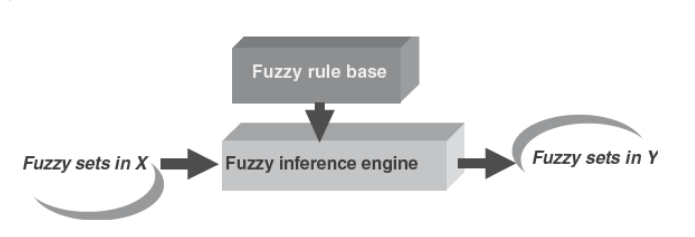
\includegraphics[scale=.40]{rbs.png}
\caption{Fig. no. 1.4, Introduction to Fuzzy
Logic using MATLAB, S.N. Sivanandam et al.}
\label{}
\end{figure}
 \end{frame}

   \section{Fuzzy Soft Set Inference System}
    \begin{frame}
    \frametitle{Decision making with Fuzzy Soft Set Inference Systems}
    
    The fuzzy soft set (F, A) denotes 'Candidates with Technical skills',\\
  $$\bordermatrix{
  \text{(F, A)} & low & medium & high  \cr
  o_1 & 0.5 & 0.2 & 0.1  \cr
  o_2 &0.1 & 0.8 & 0.1  \cr
  o_3 &0.1 & 0.2 & 0.6  \cr
  o_4 &0.2 & 0.25 & 0.3
  }$$


    \end{frame}
         \begin{frame}
  (G, B) denotes  'Candidates with Leadership skills' and,\\
  $$\bordermatrix{
  \text{(G, B)} & normal & exta-ordinary  \cr
  o_1 & 0.2 & 0.4  \cr
  o_2 &0.3 & 0.4   \cr
  o_3 &0.9 & 0.1   \cr
  o_4 &0.2 & 0.6
  }$$



  (H, C) denotes 'Candidates with Communication skills'.\\
  $$\bordermatrix{
  \text{(H, C)} & low & medium & high  \cr
  o_1 & 0.6 & 0.1 & 0  \cr
  o_2 &0.2 & 0.6 & 0.1  \cr
  o_3 &0 & 0.1 & 0.5  \cr
  o_4 &0.3 & 0.4 & 0.3
  }$$
    
 \end{frame}

 \begin{frame}
 
 \frametitle{General Form for rules}
 \begin{LARGE}
 \begin{center}
 If $A$ is $A_0$ and $B$ is $B_0$ then $C$ is $C_0$
 \end{center}
 \end{LARGE}
 \end{frame}

  \begin{frame}

    Output fuzzy soft sets on mapping some set of rules with input - \\
    \emph{Suitability for Technical Department}
      
  $$\bordermatrix{
  \text{U} & low & medium & high  \cr
  o_1 & 0.7 & 0.1 & 0  \cr
  o_2 &0 & 0.9 & 0.1  \cr
  o_3 &0.1 & 0.25 & 0.6  \cr
  o_4 &0.2 & 0.4 & 0.35
  }$$

  
  \end{frame}
  
  \begin{frame}
  \emph{Suitability for Admininstrative Department} \\
  $$\bordermatrix{
  \text{U} & low & medium & high  \cr
  o_1 & 0.1 & 0.4 & 0.3  \cr
  o_2 &0.5 & 0.2 & 0.1  \cr
  o_3 &0.6& 0.25 & 0.1  \cr
  o_4 &0.1 & 0.15 & 0.3
  }$$

  \emph{Suitability for Human Resources Department} \\
  $$\bordermatrix{
  \text{U} & low & medium & high  \cr
  o_1  &0.2 & 0.2 & 0.6  \cr
  o_2 &0 & 0.9 & 0.1  \cr
  o_3 &0.3 & 0.2 & 0.1  \cr
  o_4 &0.2 & 0.3 & 0.5
  }$$
  \end{frame}


\begin{frame}
\frametitle{Further Analysis}
\begin{itemize}
\item direct decision making from output
\item constructing comparision tables
\item aggregation
\end{itemize}
\end{frame}

\section{Strengths and Weaknesses}
\begin{frame}
\frametitle{Strengths}
\begin{itemize}
\item Easier to frame problems.
\item Simple implementation.
\item More generic/configurable in operation compared to Fuzzy inference System.
\end{itemize}
\end{frame}

\begin{frame}
\frametitle{Weaknesses}
\begin{itemize}
\item Not suitable for simple cases.
\item Needs functional expert to frame rules.
\item Rules can't be generalized.
\end{itemize}
\end{frame}


  \begin{frame}
    \frametitle{Summary}
    \begin{itemize}
    \item $\alpha$ cut on fuzzy
  parameterized fuzzy soft sets. 
  
  \item A fuzzy inference system for fuzzy soft sets.
  \end{itemize}
  \end{frame}


  
  \begin{frame}
  \frametitle{Future Work}
  The proposed algorithm can be extended for intuitionistic fuzzy soft sets.
  \end{frame}
  \bibliography{slides.bib}{}
\bibliographystyle{plain}
\end{document}
